
% Auriga theme
% https://github.com/anishathalye/auriga

\documentclass[14pt,aspectratio=169]{beamer}
\usepackage{pgfpages}
\usepackage{amsmath}
\usepackage{fancyvrb}
\usepackage{tikz}
\usetikzlibrary{arrows.meta, positioning, quotes}
\usepackage{pgfplots}

% \ifnotes
% \setbeamertemplate{note page}[plain]
% \setbeameroption{show notes on second screen=right}
% \fi

\usetheme{auriga}
\usecolortheme{auriga}

% define some colors for a consistent theme across slides
\definecolor{red}{RGB}{181, 23, 0}
\definecolor{blue}{RGB}{0, 118, 186}
\definecolor{gray}{RGB}{146, 146, 146}

\title{Universidad Nacional de La Plata (UNLP) \\ Maestría en Finanzas
  Públicas Provinciales y Municipales \\ La Politica de las Finanzas
  Públicas}
\subtitle{Clase 1}
\author{\underline{Sebastian Freille} \inst{1}}
\institute[IEF (FCE-UNC)]{\inst{1} Instituto de Economía y Finanzas (FCE-UNC)}
\date{}


\AtBeginSection[]{
    \begin{frame}
    \vfill
    \centering
    \begin{beamercolorbox}[sep=8pt,center,shadow=true,rounded=true]{title}
        \usebeamerfont{title}\insertsectionhead\par%
    \end{beamercolorbox}
    \vfill
    \end{frame}
}

%\addtobeamertemplate{headline}{}{\rule{\paperwidth}{1pt}}


\begin{document}
\maketitle


\section{Introducción, temas y enfoque}


\begin{frame}\frametitle{``Es la política, estúpido!''}
\begin{block}{Los economistas y la política}
Los economistas deben no sólo conocer sus modelos económicos, sino que
también entender de política, intereses, conflictos, pasiones, es
decir, la esencia de la vida colectiva. Por un pequeño período de
tiempo, uno puede realizar cambios a través de decretos: pero para que
ellos persistan, uno debe construir coaliciones y tener gente que los
soporte. Es decir, se debe ser un político. \\
\textit{Alejandro Foxley, ex ministro de Finanzas de Chile}
\end{block}
\end{frame}


\begin{frame}\frametitle{Economía política}
\begin{itemize}
\item Economía $\longrightarrow$ uso óptimo de recursos escasos
\item Política $\longrightarrow$ estudio del poder y la autoridad
\item Poder $\longrightarrow$ habilidad (capacidad) de individuos y/o
  grupos para lograr sus objetivos
\item En cualquier estudio que pretenda describir la complejidad de
  las relaciones sociales en sus dimensiones económicas y políticas,
  estos elementos deben analizarse en forma conjunta.
\end{itemize}
\end{frame}


\begin{frame}\frametitle{Economía política: Ayer y hoy}
\begin{itemize}
\item La economía como disciplina nace y se desarrolla como economía
  política (Smith, Ricardo, Marx, JS Mill, Say). La economia
  neoclásica enfoca en \textbf{planificador benevolente}
  $\longrightarrow$ enfoque normativo 
  \item ¿Cómo y porqué es la política económica como es? ¿Cómo es el
    proceso político de toma de decisiones colectivas por parte de
    \textbf{agentes con preferencias diferentes} $\longrightarrow$
    enfoque positivo
    \item Esto último es lo que se entiende modernamente por \textbf{economia política}
\end{itemize}
\end{frame}



\begin{frame}
\frametitle{Economía política: Orígenes}
\begin{itemize}
  \item Existen tres tradiciones que convergen en la economia política
    \begin{itemize}
    \item Teoría de la \textbf{política macroeconómica} $\longrightarrow$ expectativas racionales, incentivos del \textit{policy maker} y comportamiento estratégico. Eminentemente teórica; instituciones políticas poco realistas
\item Teoría de la \textbf{elección pública} $\longrightarrow$ finanzas públicas, política regulatoria. Eje: problema de agencia entre el gobierno (agente) y ciudadanos (principal). 
\item Teoría de la \textbf{elección social} $\longrightarrow$ modelos formales de análisis político. Se inicia con los modelos de votación espacial y la teoría axiomática de la elección social (Arrow). Estudia decisiones colectivas en instituciones políticas específicas.
\end{itemize}
\end{itemize}
\end{frame}


\begin{frame}\frametitle{Economía política: Metodología}
\begin{block}{Enfoque de la economía política moderna: síntesis}
Utiliza el enfoque de equilibrio general de la \textbf{teoría macroeconómica}
de la política y explota las herramientas de la \textbf{teoría de la elección
racional} para el análisis de los problemás principales de la \textbf{teoría
de la elección pública}
\end{block}
\end{frame}


\begin{frame}\frametitle{Economía política: Metodología (cont.)}
  \begin{itemize}
    \item Enfoque consiste en aplicar métodos de análisis modernos al
      ámbito político $\longrightarrow$ politicas económicas resultado
      de interacción entre individuos racionales con preferencias
      heterogéneas
      \item Si bien el método en ocasiones suele ser criticado por
        excesivamente formal y racionalista, se pueden incorporar
        otros paradigmas para analizar el efecto de relajar ciertos supuestos.
\end{itemize}
\end{frame}




\begin{frame}\frametitle{Economía política: Temas y ejes}
  \begin{itemize}
    \item ¿Cuál es el origen de la enorme variabilidad en las políticas
económicas entre países y a lo largo de los años?
\item ¿Cuál es la manera en que distintos conjuntos de reglas sociales y de
organizaciones económicas afectan el comportamiento, la asignación de
recursos y los resultados de equilibrio?
\item ¿Cómo cambian estas reglas y organizaciones en el tiempo y entre países?
\end{itemize}
\end{frame}



\begin{frame}\frametitle{Economía política: Las tres I's}
\begin{block}{Intereses}
Representados por preferencias de diferentes agentes por alternativas
de políticas. Se modelan al nivel individual
\end{block}
  \begin{block}{Instituciones}
Restricciones creadas por los humanos que estructuran la interacción
económica, política y social.
\end{block}
\begin{block}{Ideas}
Incluyen paradigmas, sentimientos públicos, programas y encuadres que
moldean e impactan el tipo y forma de las decisiones adoptadas
\end{block}
 \note{
    El análisis de los intereses supone que siempre existe un problema
 bien definido de optimización que incluye una función objetivo, una
 serie de restricciones y un conjunto de alternativas. Esto suele ser
 un supuesto limitante ya que en muchas situaciones esto no se
 cumple.

 Las instituciones incluyen tanto restricciones informales (codigos de
 conducta, costumbres, tradiciones) como restricciones formales
 (constituciones, leyes, derechos de propiedad). Las instituciones
 pueden ser exógenas y endogenas.

 Algunos ejemplos de ideas que en economía han tenido impacto sobre
 las políticas adoptadas --supply-side economics; modern monetary
 theory; consenso de Washington. 
  }
\end{frame}




\begin{frame}{Economía y política: Politicas economicas}
 \begin{figure}
    \centering
    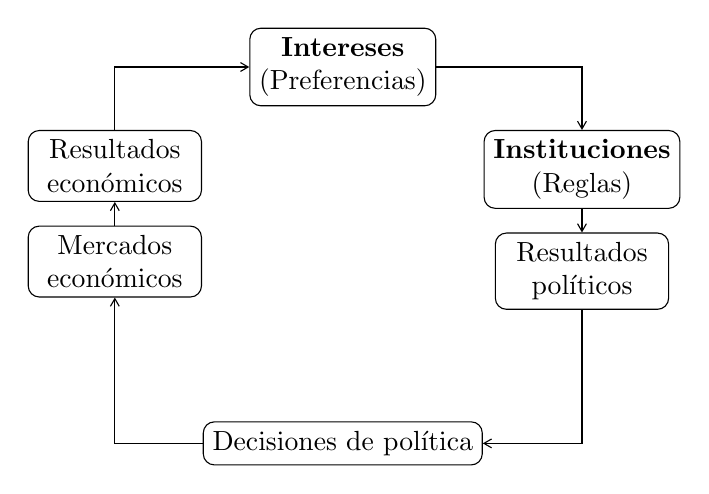
\begin{tikzpicture}[
node distance = 3mm and 6mm, 
   box/.style = {draw, rounded corners, 
                 minimum width=22mm, minimum height=5mm, align=center},
            > = {Straight Barb[angle=60:2pt 3]},
   bend angle = 15,
         auto = right,
         ]
\node (n1)  [box] {\textbf{Intereses} \\ (Preferencias)};
\node (n2)  [box, below right=of n1]    {\textbf{Instituciones} \\ (Reglas)};
\node (n3)  [box, below left=of n1]    {Resultados \\ económicos};
\node (n4)  [box, below=of n2]    {Resultados \\ políticos};
\node (n5)  [box, below=of n3]    {Mercados \\ económicos};
\node (n6)  [box, below=4cm of n1]    {Decisiones de política};

%
\draw[->] (n1) -| (n2);
\draw[->] (n2) -- (n4);
\draw[->] (n4) |- (n6);
\draw[->] (n6) -| (n5);
\draw[->] (n5) -- (n3);
\draw[->] (n3) |- (n1);
    \end{tikzpicture}
 %   \caption{Decisiones de politica en la economía política}
  \end{figure}

  \note{
    Here's a note for this slide.
  }
\end{frame}





\section{Heterogeneidad en politicas y resultados económicos}



\begin{frame}\frametitle{Politica económica comparada}
  \begin{itemize}
    \item Existe una relación positiva entre gasto público y PIB per
      capita con alguos \textit{outliers} y posibles no linearidades
      \item ¿Cómo se explican estas diferencias desde un enfoque
        puramente económico sin considerar la politica?
        \item Posibles explicaciones $\longrightarrow$ 1) mayor rol
          redistributivo del Estado; 2) instituciones políticas
          --presidencialismo vs parlamentarismo, mayoritario vs
          representación proporcional.
          \end{itemize}
\end{frame}


\begin{frame}\frametitle{Politica económica comparada (cont.)}
  \begin{figure}[htbp]
    \centering
    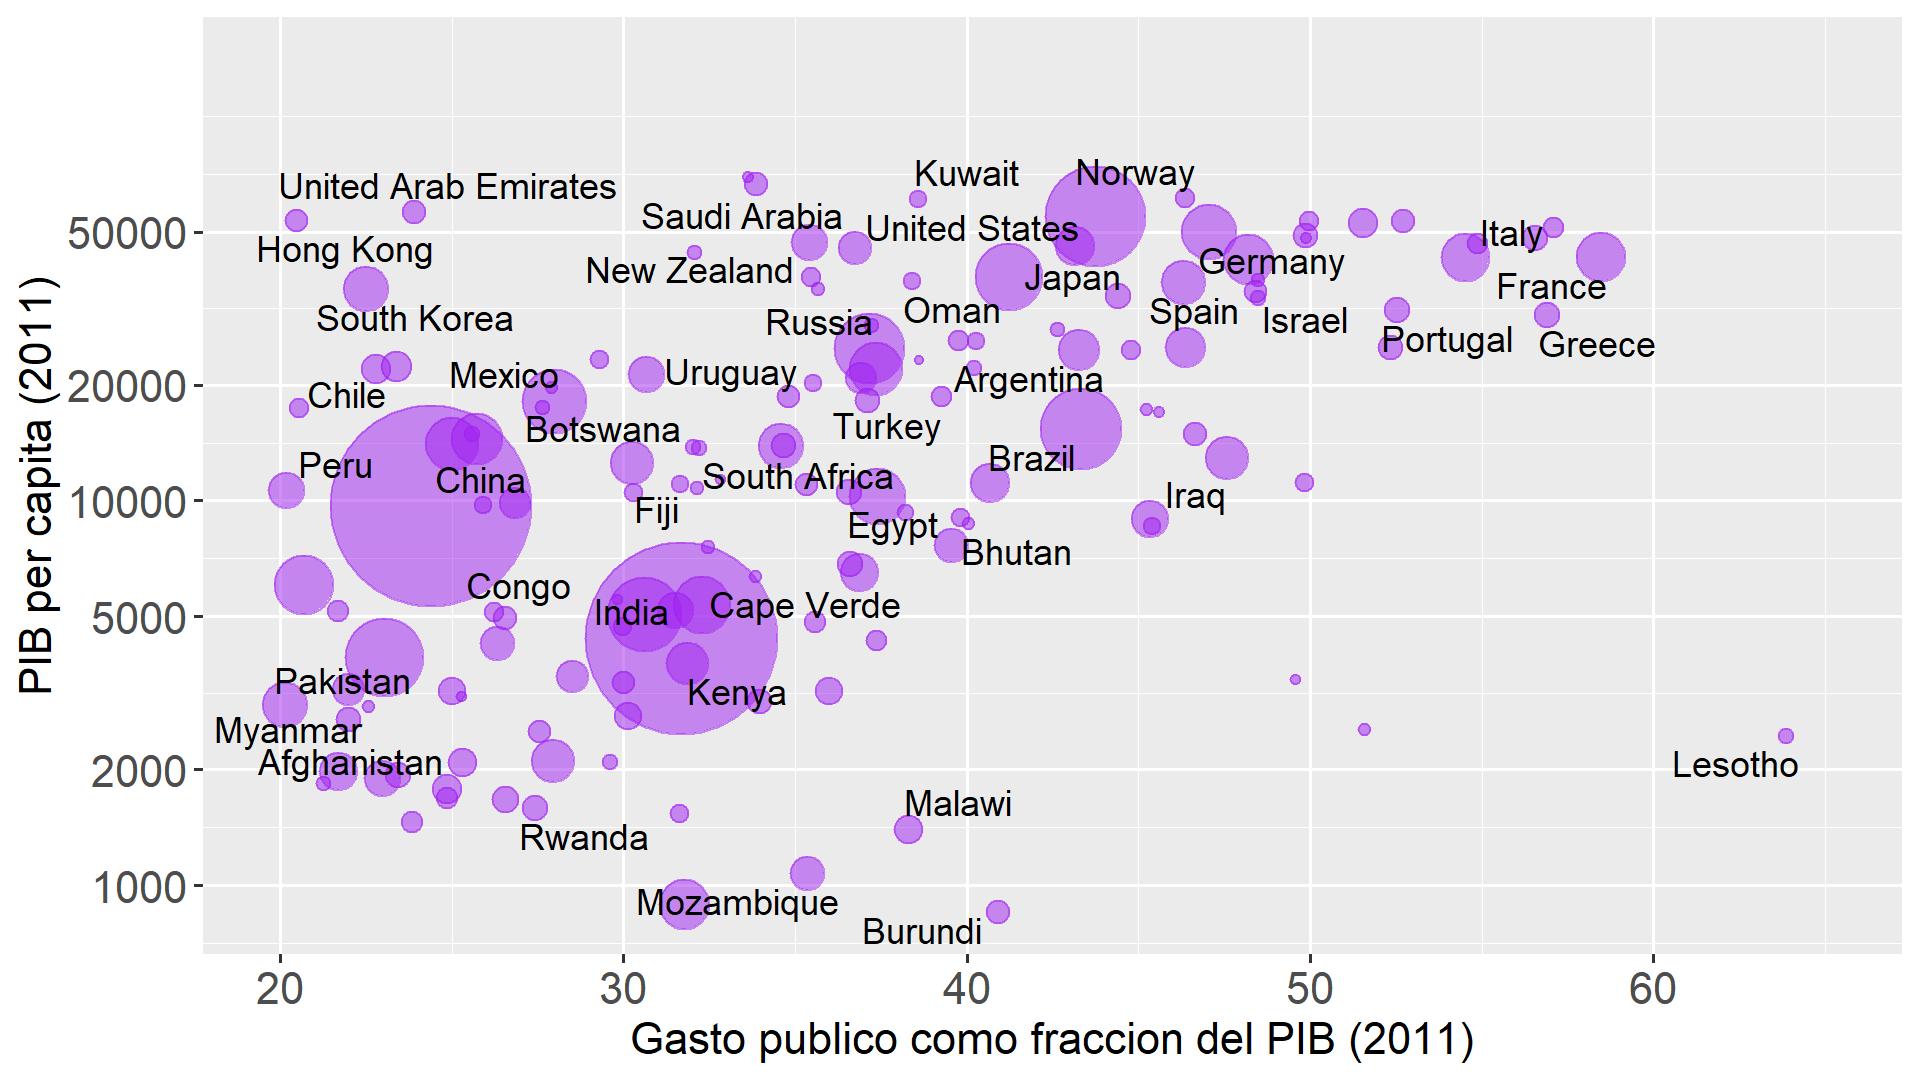
\includegraphics[scale=0.4]{fig01}
    \caption{Gasto público ($\%PIB$) y PBI per capita}
    \label{fig:3}
  \end{figure}
\end{frame}


\begin{frame}\frametitle{Politica económica comparada (cont.)}
  \begin{itemize}
    \item Si miramos evolución comparada de largo plazo, observamos claras tendencias
      a mayor participación estatal en la economía $\longrightarrow$
      medido tanto por el lado de gastos como de recursos y también
      para diferentes países
      \item También aquí la política es importante $\longrightarrow$
        expansión y fortalecimiento de las democracias en los últimos
        150 años
        \item ¿Diferentes preferencias? ¿Diferentes instituciones?
          \end{itemize}
\end{frame}


\begin{frame}\frametitle{Política económica comparada (cont.)}
  \begin{figure}[htbp]
    \centering
    \includegraphics[scale=0.4]{fig03}
    \caption{Evolución gasto público ($\%PIB$) - Paises industriales}
    \label{fig:4}
  \end{figure}
\end{frame}



\begin{frame}\frametitle{Política económica comparada (cont.)}
  \begin{figure}[htbp]
    \centering
    \includegraphics[scale=0.4]{fig05}
    \caption{Evolución gasto público ($\%PIB$) - Países en desarrollo}
    \label{fig:5}
  \end{figure}
\end{frame}






\begin{frame}\frametitle{Politica económica comparada (cont.)}
  \begin{itemize}
    \item Países pobres versus ricos con similar recaudación tributaria --ie tamaño del
      Estado- $\longrightarrow$ Lesotho/Alemania
      \item Países con similar riqueza pero diferente rol del Estado
        $\longrightarrow$ Oman y Arabia Saudita / EEUU / Noruega
        \item Economia puede explicar algunas diferencias
          $\longrightarrow$ ley de Wagner, efecto ``umbral''
        \item Varias teorias explicativas desde el estudio de la
          política $\longrightarrow$ 1) maldición de los recursos, 2)
          corrupción, 3) incentivos político-electorales 
          \end{itemize}
\end{frame}



\begin{frame}\frametitle{Política económica comparada (cont.)}
  \begin{figure}[htbp]
    \centering
    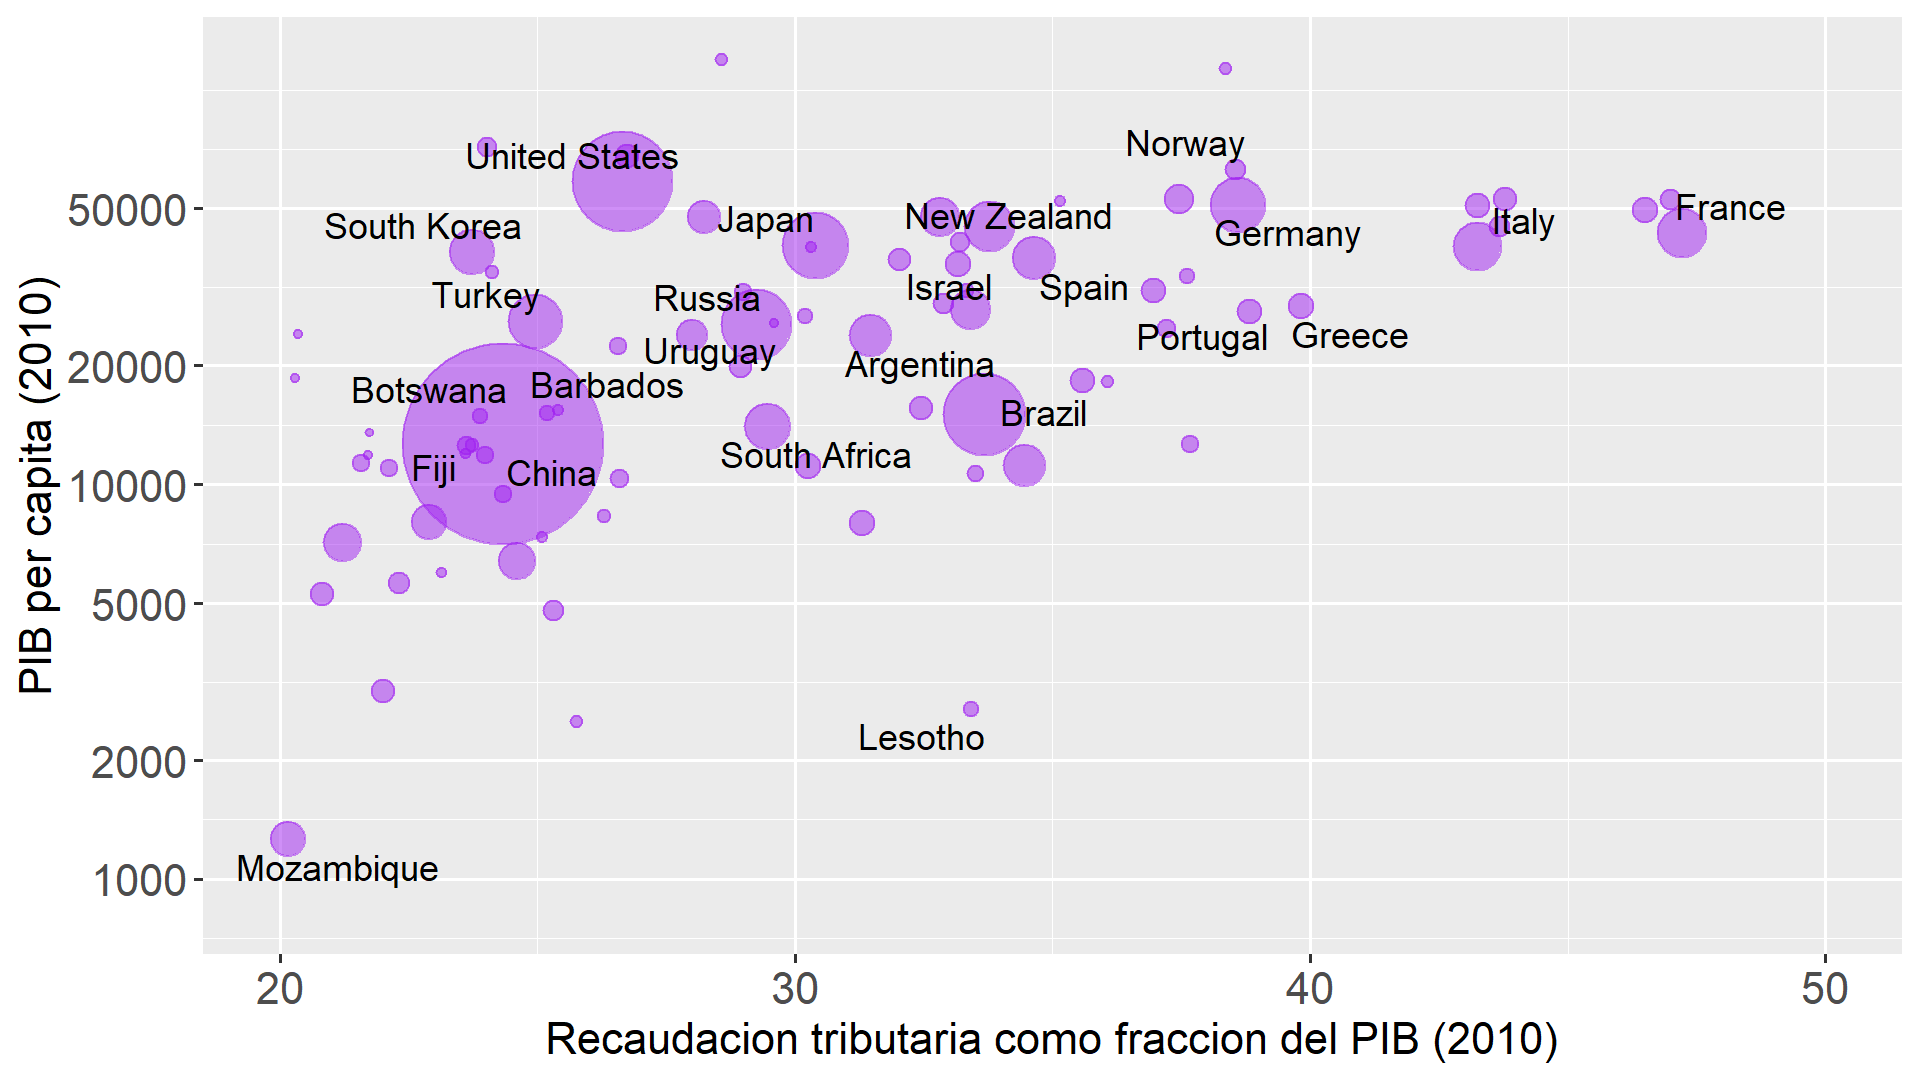
\includegraphics[scale=0.4]{fig02}
    \caption{Recaudacion tributaria ($\%PIB$) y PBI per capita}
    \label{fig:1}
  \end{figure}
\end{frame}


  
\begin{frame}\frametitle{Política económica comparada (cont.)}
  \begin{figure}[htbp]
    \centering
    \includegraphics[scale=0.4]{fig04}
    \caption{Evolución recaudación tributaria ($\%PIB$) - Paises industriales}
    \label{fig:1}
  \end{figure}
\end{frame}


\section{Aplicación: Equilibrio sin y con política}




\begin{frame}{Aplicación: el rol de la política}
  \begin{itemize}
    \item Un aspecto relevante de la política es en lo que hace a la \textbf{heterogeneidad de
        intereses}
      \item Restricciones políticas derivadas de ello implica que las políticas adoptadas en la práctica \textbf{no
          son óptimas}
        \item Implicaciones positivas $\longrightarrow$ si la política
          óptima se encuentra no resulta cierto que esta se implementa
          (implícito en la \textit{economía del bienestar})
          \item Implicaciones normativas $\longrightarrow$ ¿cómo
            pueden diseñarse instituciones y políticas para lograr
            ciertos objetivos?
            \end{itemize}

  \note{
    Here's a note for this slide.
  }
\end{frame}


\begin{frame}{Aplicación: Equilibrio sin política}
  \begin{itemize}
  \item Basado en Drazen (2000) y Ferguson/Querubin (2018)
    \item Suponga un \textbf{individuo representativo}, Ana quien debe elegir
      cuánto destinar de sus recursos iniciales $A_{o}$ para sus
      vacaciones de este año y el próximo
      \item  Note que no hay problema político (no conflicto
        de intereses) sino uno técnico
        \item ¿Cuál es la manera óptima de dividir los recursos entre
          dos vacaciones (presente y futuro)?
    
  \end{itemize}

  \note{
    Here's a note for this slide.
  }
\end{frame}




\begin{frame}{Aplicación: Equilibrio sin política (cont.)}
  \begin{itemize}
  \item Sea $u(x_{t})$ la utilidad de Ana por destinar $x$ a sus
    vacaciones en $t$ con $u'>0$ y $u''<0$. El parámetro $\beta$
    compara utilidades en distintos momentos --una unidad de utilidad
    hoy es igual a $\beta$ unidades de utilidad mañana [$0<\beta<1$]
  \item Problema:
    \begin{equation*}
      \max_{x_{t},x_{t+1},s} u(x_{t})+\beta u(x_{t+1})
    \end{equation*}
  \item sujeto a:
    \begin{align*}
      A_{0}(1-s)&=x_{t} \\

     sA_{0}(1+r_{t})&=x_{t+1} 
      \end{align*}
    \end{itemize}

  \note{
    Here's a note for this slide.
  }
\end{frame}



\begin{frame}{Aplicación: Equilibrio sin política (cont.)}
  \begin{itemize}
  \item Sustituyendo las restricciones:
    \begin{equation*}
\max_{x_{t}}u(x_{t})+\betau((A_{o}-x_{t})(1+r_{t})) 
\end{equation*}
\item Y la  solución de esto es:
  \begin{equation*}
u'(x_{t})=\beta(1+r_{t})u'(x_{t+1})
\end{equation*}
\item ¿Interpretación de esta solución (ecuación de Euler)?
    \end{itemize}

  \note{
    Here's a note for this slide.
  }
\end{frame}



\begin{frame}{Aplicación: Equilibrio con política}
  \begin{itemize}
  \item \textbf{Con individuos heterogéneos ex-ante} $\longrightarrow$
    preferencias diferentes por consumo presente/futuro [dos tipos de heterogeneidad: \textit{ex
      ante} y \textit{ex post}]
    \item Los recursos son los mismos que antes pero ahora hay dos
      individuos, Ana (A) y Juan (J) y sea $\beta^{A}>\beta^{J}$ [Juan
      es más impaciente que Ana]
      \item Problema $\longrightarrow$ maximizar la función de
        bienestar social (suma ponderada de utilidades individuales)
        $\longrightarrow$ $\alpha$ ponderación de cada individuo
        
    \end{itemize}

  \note{
    Here's a note for this slide.
  }
\end{frame}


\begin{frame}{Aplicación: Equilibrio con política (cont.)}
  \begin{itemize}
  \item Problema (neoclasico):
    \begin{equation*}
\max_{x_{t},x_{t+1},s} \alpha\left[u(x_{t})+\beta^{A}u(x_{t+1})\right] + (1-\alpha)\left[u(x_{t})+\beta^{J}u(x_{t+1})\right]
\end{equation*}
\item sujeto a:
  \begin{equation*}
A_{0}=x_{t}+\frac{x_{t+1}}{(1+r_{t})}
\end{equation*}
\item si el bien ``vacaciones'' es no rival --unica fuente de conflicto
  la diferencia ex-ante en el grado de impaciencia de cada uno 
    \end{itemize}

  \note{
    Here's a note for this slide.
  }
\end{frame}



\begin{frame}{Aplicación: Equilibrio con política (cont.)}
  \begin{itemize}
  \item Sustituyendo las restricciones:
    \begin{equation*}
u'(x_{t})=(1+r_{t})[\alpha \beta^{A}+(1-\alpha)\beta^{J}]u'(x_{t+1})
\end{equation*}
\item Para diferentes $\alpha$ trazamos \textbf{curva de contrato} con
  asignaciones de $x_{t}$ y $x_{t+1}$ eficientes en sentido de Pareto
  \item Varios problemas con esto: 1) cada persona requiere un
    $\alpha$ mas alto, 2) ¿cómo se determina $\alpha$, 3) ¿cómo afecta
    el valor de $\alpha$ a la asignación de recursos, 4) ¿estaremos
    sobre la curva de contrato?
    \end{itemize}

  \note{
    Here's a note for this slide.
  }
\end{frame}


\begin{frame}{Aplicación: Equilibrio con política (cont.)}
  \begin{itemize}
  \item \textbf{Sin individuos heterogéneos ex-ante} $\longrightarrow$
    problema converge al del individuo representativo PERO las
    vacaciones no son un bien no rival. El problema es:
     \begin{align*}
\max_{x_{t},x_{t+1},s} & \alpha\left[u(\lambda x_{t})+\beta u(\lambda
      x_{t+1})\right] \\ & +(1-\alpha)\left[u((1-\lambda) x_{t})+\beta u((1-\lambda) x_{t+1})\right]
      \end{align*}
    \item sujeto a [$\lambda$ porcentaje que disfruta Juan del gasto $x$]
      \begin{align*}
                A_{0}(1-s)&=x_{t}=\lambda x_{t}+(1-\lambda)x_{t} \\
        sA_{0}(1+r_{t})&=x_{t+1}=\lambda x_{t+1}+(1-\lambda)x_{t+1} 
      \end{align*}
    \end{itemize}

  \note{
    Here's a note for this slide.
  }
\end{frame}


\begin{frame}{Aplicación: Equilibrio con política (cont.)}
  \begin{itemize}
  \item Resolviendo:
    \begin{align*}
\alpha \lambda u'(\lambda
      x_{t})+(1-\alpha)(1-\lambda)u'((1-\lambda)x_{t})= \\
      \beta(1+r_{t})\left[\alpha \lambda u'(\lambda
      x_{t+1})+(1-\alpha)(1-\lambda)u'((1-\lambda)x_{t+1})\right]
    \end{align*}
      \item Note que $\alpha$ es crucial $\longrightarrow$ pero ahora
        $\lambda$ también lo es [aún suponiendo que $\alpha=0.5$
        existe conflicto de interés]
        \begin{align*}
\lamdba u'(\lambda
          x_{t})+(1-\lambda)u'((1-\lambda)x_{t})= \\
          \beta(1+r_{t})\left[\lambda u'(\lambda
      x_{t+1})+(1-\lambda)u'((1-\lambda)x_{t+1})\right]
          \end{align*}
\item Si $\lambda=1$, el resultado seria preferido por Juan y si
  $\lambda=0$ el resultado sería preferido por Ana. 
        \end{itemize}

  \note{
    Here's a note for this slide.
  }
\end{frame}


\begin{frame}{Aplicación: Equilibrio con política (cont.) }
  \begin{itemize}
    \item Cuando no hay heterogeneidad, el problema es trivial
      $\longrightarrow$ problema técnico depende de parámetros
      subjetivos
      \item Cuando hay heterogeneidad en preferencias (\textit{ex ante}) $\longrightarrow$ como se ponderan utilidades
      individuales [$\alpha$ exógeno]
      \item Cuando hay heterogeneidad en distribución (\textit{ex
          post}) $\longrightarrow$ como se
        ponderan utilidades invididuales y como se
        distribuye/asigna las cantidades consumidas del
        bien
        \item ¿Cómo se determinan los parámetros $\alpha$ y $\lambda$
          en la práctica? No a través del mercado sino del proceso político
  \end{itemize}

  \note{
    Here's a note for this slide.
  }
\end{frame}



\section{Economía y politica: Dos sistemas}


\begin{frame}{Economía y política: Dos sistemas}
  \begin{itemize}
    \item Una persona, un voto $\longrightarrow$ \textbf{democracia}
    \item Un dólar, un voto $\longrightarrow$ \textbf{mercado}
      \item Función objetivo del gobierno incluye ambos
      \begin{align}
        G&=f(W,C)=\alpha W+\sum_{i}C_{i}
        \end{align}
        \item $W$ es bienestar agregado; $C_{i}$ es dinero aportado por grupo $i$
      --$\alpha$ ponderador del bienestar agregado. 
  \end{itemize}

  \note{
    Here's a note for this slide.
  }
\end{frame}


\begin{frame}{Economía y política: Dos sistemas (cont.)}
 \begin{figure}
    \centering
    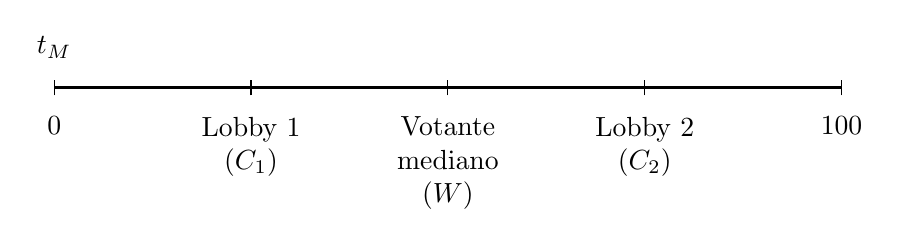
\begin{tikzpicture}[scale=0.5]
  \draw [thick] (0,0) -- (20,0);
\draw (0,-.2) -- (0, .2);
\draw (5,-.2) -- (5, .2);
\draw (10,-.2) -- (10, .2);
\draw (15,-.2) -- (15, .2);
\draw (20,-.2) -- (20, .2);
\node[align=center, above] at (0,+.5)%
{$t_{M}$};
\node[align=center, below] at (0,-.5)%
{$0$};
\node[align=center, below] at (5,-.5)%
{Lobby 1\\ $(C_{1})$};
\node[align=center, below] at (10,-.5)%
{Votante\\ mediano\\ $(W)$};
\node[align=center, below] at (15,-.5)%
{Lobby 2\\ $(C_{2})$};
\node[align=center, below] at (20,-.5)%
{$100$};
    \end{tikzpicture}
    \caption{Preferencias en el espacio}
  \end{figure}

  \note{
    Here's a note for this slide.
  }
\end{frame}




\section{Recapitulando}

\begin{frame}{Conclusiones}
  \begin{itemize}
    \item La política económica en las sociedades modernas no puede
      explicarse sólamente en base a teorías y evidencias económicas
      $\longrightarrow$ introducir la política explícitamente en el análisis
      \item Hay varias formas de introducir la política
        $\longrightarrow$ optamos por la aproximación de la nueva
        economia política
        \item Pondremos el énfasis en algunos sencillos modelos
          teóricos --de comportamiento-- pero ilustraremos el análisis
          con evidencias empíricas
  \end{itemize}

  \note{
    Here's a note for this slide.
  }
\end{frame}



\end{document}



\end{document}
